\documentclass[tikz,border=2pt]{standalone}
\usepackage{amsmath}
\usetikzlibrary{arrows.meta}
\begin{document}
% ifelse(x > 0, x^2, -x) for x = c(-2, 2): element 1 (test FALSE) is taken from -x = 2,
% element 2 (test TRUE) from x^2 = 4; the result is c(2, 4). Unused cells are grey.
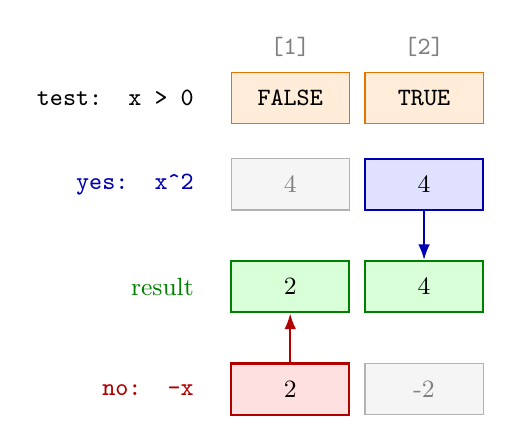
\begin{tikzpicture}[font=\small, >={Latex[length=2mm]},
  cell/.style={draw, minimum width=1.5cm, minimum height=6.5mm, inner sep=2pt},
  lab/.style={anchor=east}]
  % index labels
  \node[gray] at (1,0.65) {\texttt{[1]}};
  \node[gray] at (2.7,0.65) {\texttt{[2]}};
  % test row
  \node[lab] at (-0.1,0) {\texttt{test: x > 0}};
  \node[cell, fill=orange!15, draw=orange!90!black] at (1,0)   {\texttt{FALSE}};
  \node[cell, fill=orange!15, draw=orange!90!black] at (2.7,0) {\texttt{TRUE}};
  % yes row
  \node[lab, blue!70!black] at (-0.1,-1.1) {\texttt{yes: x\^{}2}};
  \node[cell, draw=gray!60, fill=gray!8, text=gray] (y1) at (1,-1.1) {4};
  \node[cell, draw=blue!70!black, fill=blue!12, thick] (y2) at (2.7,-1.1) {4};
  % result row
  \node[lab, green!50!black] at (-0.1,-2.4) {result};
  \node[cell, draw=green!50!black, fill=green!15, thick] (o1) at (1,-2.4) {2};
  \node[cell, draw=green!50!black, fill=green!15, thick] (o2) at (2.7,-2.4) {4};
  % no row
  \node[lab, red!70!black] at (-0.1,-3.7) {\texttt{no: -x}};
  \node[cell, draw=red!70!black, fill=red!12, thick] (n1) at (1,-3.7) {2};
  \node[cell, draw=gray!60, fill=gray!8, text=gray] (n2) at (2.7,-3.7) {-2};
  % selections
  \draw[->, thick, blue!70!black] (y2) -- (o2);
  \draw[->, thick, red!70!black] (n1) -- (o1);
\end{tikzpicture}
\end{document}
